% ReRoom -- relation-conditioned DiT backbone (paper-figure style).
\documentclass[border=6pt]{standalone}
\usepackage{tikz}\usepackage{amsmath,amssymb}\usepackage{pifont}
\usetikzlibrary{arrows.meta,positioning,fit,backgrounds,calc}
\definecolor{ink}{HTML}{1A1A1A}\definecolor{mut}{HTML}{6B7280}
\definecolor{net}{HTML}{3B5BD9}\definecolor{prj}{HTML}{E8770F}
\tikzset{
  slbl/.style ={font=\tiny,text=mut},
  tok/.style  ={draw=ink,line width=.5pt,fill=white,align=center,font=\scriptsize,inner sep=3pt,minimum width=42mm},
  mod/.style  ={draw=ink,line width=.5pt,rounded corners=2pt,fill=white,align=center,font=\scriptsize,inner sep=4pt,minimum width=46mm,text=ink},
  acc/.style  ={draw=net,line width=.9pt,rounded corners=2pt,fill=net!7,align=center,font=\scriptsize,inner sep=4pt,minimum width=46mm,text=ink},
  flw/.style  ={draw=prj,line width=.9pt,rounded corners=2pt,fill=prj!7,align=center,font=\scriptsize,inner sep=4pt,text=ink},
  cnd/.style  ={draw=mut,line width=.5pt,rounded corners=2pt,fill=mut!5,align=center,font=\scriptsize,inner sep=3pt,text=ink},
  a/.style    ={-{Stealth[length=4.5pt]},line width=.8pt,ink},
  ad/.style   ={-{Stealth[length=3.5pt]},line width=.6pt,dashed},
}
\begin{document}
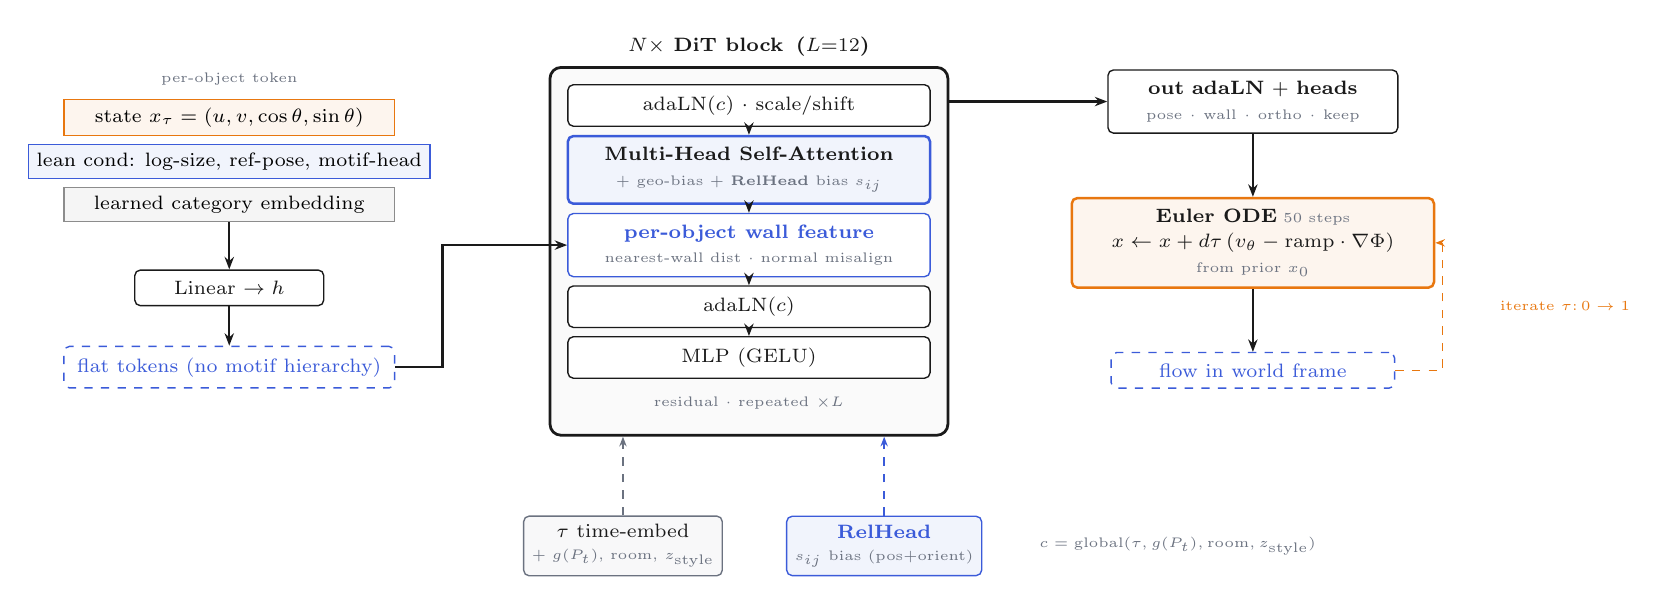
\begin{tikzpicture}
% ===== token stack (left) =====
\node[tok,fill=prj!7,draw=prj] (t1) at (0,2.0) {state $x_\tau=(u,v,\cos\theta,\sin\theta)$};
\node[tok,fill=net!7,draw=net,below=1mm of t1] (t2) {lean cond: log-size, ref-pose, motif-head};
\node[tok,fill=black!4,draw=black!45,below=1mm of t2] (t3) {learned category embedding};
\node[slbl,above=0.5mm of t1] {per-object token};
\node[mod,minimum width=24mm,below=6mm of t3] (lin) {Linear $\to h$};
\node[mod,minimum width=42mm,draw=net,dashed,text=net,below=5mm of lin] (flat) {flat tokens (no motif hierarchy)};
\draw[a] (t3) -- (lin); \draw[a] (lin) -- (flat);

% ===== DiT block (center) =====
\def\bx{6.6}
\node[mod] (m1) at (\bx,2.15) {adaLN$(c)$ $\cdot$ scale/shift};
\node[acc,below=1mm of m1] (m2) {\textbf{Multi-Head Self-Attention}\\[1pt]{\tiny\color{mut} $+$ geo-bias $+$ \textbf{RelHead} bias $s_{ij}$}};
\node[mod,draw=net,text=net,below=1mm of m2] (m3) {\textbf{per-object wall feature}\\[1pt]{\tiny\color{mut} nearest-wall dist $\cdot$ normal misalign}};
\node[mod,below=1mm of m3] (m4) {adaLN$(c)$};
\node[mod,below=1mm of m4] (m5) {MLP (GELU)};
\draw[a] (m1)--(m2);\draw[a] (m2)--(m3);\draw[a] (m3)--(m4);\draw[a] (m4)--(m5);
\node[slbl,below=1mm of m5] (res) {residual $\cdot$ repeated $\times L$};
\begin{scope}[on background layer]
  \node[draw=ink,line width=1pt,rounded corners=4pt,fill=black!2,fit=(m1)(m2)(m3)(m4)(m5)(res),inner sep=6pt,
        label={[ink,font=\scriptsize\bfseries]above:$N\times$ DiT block \,($L{=}12$)}] (blk) {};
\end{scope}
\draw[a] (flat.east) -- ++(0.6,0) |- (m3.west);

% ===== conditioning (below) =====
\node[cnd,below=10mm of blk.south,anchor=north,xshift=-16mm] (tau)
  {$\tau$ time-embed\\{\tiny\color{mut} $+\;g(P_t)$, room, $z_\text{style}$}};
\node[cnd,draw=net,fill=net!7,right=8mm of tau] (rh) {\textbf{\textcolor{net}{RelHead}}\\{\tiny\color{mut} $s_{ij}$ bias (pos$+$orient)}};
\draw[ad,mut] (tau.north) -- (tau.north|-blk.south);
\draw[ad,net] (rh.north) -- (rh.north|-blk.south);
\node[slbl,right=6mm of rh,align=left] {$c=\text{global}(\tau,g(P_t),\text{room},z_\text{style})$};

% ===== output heads + ODE (right) =====
\node[mod,minimum width=36mm,text width=34mm] (heads) at (13.0,2.2) {\textbf{out adaLN $+$ heads}\\[1pt]{\tiny\color{mut} pose $\cdot$ wall $\cdot$ ortho $\cdot$ keep}};
\node[flw,minimum width=46mm,below=8mm of heads] (ode)
  {\textbf{Euler ODE}\;{\tiny\color{mut} 50 steps}\\[1pt]$x\leftarrow x+d\tau\,(v_\theta-\text{ramp}\cdot\nabla\Phi)$\\[1pt]{\tiny\color{mut} from prior $x_0$}};
\node[mod,draw=net,dashed,text=net,minimum width=36mm,below=8mm of ode] (world) {flow in world frame};
\draw[a] (blk.east|-heads) -- (heads.west);
\draw[a] (heads) -- (ode);
\draw[a] (ode) -- (world);
\draw[ad,prj] (world.east) -- ++(6mm,0) |- (ode.east);
\node[slbl,prj,anchor=west] at ($(ode.east)+(7mm,-8mm)$) {iterate $\tau{:}\,0\to1$};
\end{tikzpicture}
\end{document}
